\documentclass[a4paper, 10pt, final, garamond]{book}
\usepackage{cours-preambule}

\titleformat{\item}{}{\arabic{item})}{.5em}{}{}
\titleformat{\subitem}{}{\arabic{item}) \alph{subitem} --}{.5em}
{}{}

\makeatletter
\renewcommand{\@chapapp}{Devoir surveill\'e -- num\'ero}
\makeatother

\begin{document}
\setcounter{chapter}{1}

\chapter{Commentaires sur le DS n°2}

\section{Commentaires généraux}

Très grande disparité pour ce DS. Certaimes ne savent pas appliquer la loi des
mailles, d'autres ne jurent que par la loi d'Ohm apprise en classe 4\ieme, quand
d'autres vont presque au bout du sujet. Globalement c'est quand même pas
désastreux, mais j'ai vu de l'énergie se créer de nulle part, \textbf{beaucoup}
de condensateurs briser la causalité et remonter dans le temps, des tensions
être des courants, des diviseurs de tension devenir des multiplicateurs de
tension… Ça manque énormément de recul et surtout de commentaires de votre part
sur la pertinence physique de ce que vous écrivez. Un malus «~notation~» (par
rapport aux notations de l'énoncé) et un malus «~physique~» par rapport à la
logique de vos équations seront appliqués à partir du prochain DS. Voyons le
détail.

% Il y a plus d'écart de points entre la première personne et la troisième que de
% points cumulé des 3 dernierz.

\section{Exercice 1 \hfill \textcolor{red}{/34}}

\textbf{La consigne était pourtant claire~: les résultats étaient demandés en
fonction de $E$ et $R$ uniquement}, sauf question 4. Donc des résultats avec
$U_1$ ou avec $I$…

\begin{enumerate}
    \item Très proche du cours et des exercices. On faisait des résistances
        équivalentes de proche en proche, à partir de la droite. \textbf{Il
        fallait faire les schémas équivalents}. Il y avait aussi des points pour
        dire $\mathbf{12R\parr 4R}$ ou $\mathbf{3R}$\textbf{ série avec
        }$\mathbf{2R}$. Par rapport au corrigé, nous n'avions pas vu la loi de
        \textsc{Pouillet}, dans ma notation c'était LdM + Ld$\Omega$. \textbf{La
        loi d'Ohm ne s'applique pas à un générateur}. Attention à l'homogénéité.
        \hfill \textcolor{ForestGreen}{/16}

    \item Attention, $U$ n'est pas «~la tension dessinée à droite~». Le concept
        de tension est encore mal compris. La tension $U$ disparaît avec les
        résistances équivalents successives. Il fallait voir que $U_1$ était la
        tension de la branche de gauche mais aussi celle de $20R$ puisqu'elles
        sont en parallèle. Par contre, vous ne pouvez pas extraire une maille
        qui vous intéresse pour travailler dessus, ça ne marche pas comme ça,
        mais il y avait des points pour le schéma sur lequel vous travailliez
        (pas trop pénalisé quand les premiers étaient bien fait et bien
        référencés).
        \hfill \textcolor{ForestGreen}{/4}

    \item À partir de $U$ le plus simple c'est la loi d'Ohm. Mais même si
        c'était écrit «~méthode de votre choix~» et que vous avez choisi
        d'utiliser des ponts diviseurs de courant, il fallait répondre à la
        question 4. Quand c'était mélangé, j'ai fait en sorte de répartir les 9
        points des questions 3 et 4 correctement. \hfill
        \textcolor{ForestGreen}{/5}

    \item Des difficultés avec le pont diviseur de courant. Points pour le
        recopiage du schéma utilisé. Si on vous demande de vérifier,
        \textbf{concluez} sur le fait que ça marche. \hfill
        \textcolor{ForestGreen}{/4}

    \item Rien de particulier. $P_G = EI$. \hfill \textcolor{ForestGreen}{/2}

    \item Pas de commentaire particulier. \hfill \textcolor{ForestGreen}{/3}
\end{enumerate}

\section{Exercice 2\hfill \textcolor{red}{/32}}

\begin{enumerate}
    \item Le terme «~potentiel~» n'a été que peu compris, et l'ordre des
        soustractions mal géré. \hfill \textcolor{ForestGreen}{/2}

    \item Les lois de \textsc{Kirchhoff} ne sont pas les ponts diviseurs. \hfill
        \textcolor{ForestGreen}{/10}

    \item Si vous faites des simplifications, faites les schémas équivalents~!
        Des points pour dire «~$R_1$ et $R_2$ en série~». Une réponse encadrée
        ne peut s'arrêter à une notation que vous avez introduite~: il y avait
        un point pour $I = E/R_{\rm eq}$ \textbf{et} pour $I = E\frac{R_1 + R_2 +
        R_3 + R_4}{(R_1+R_2)(R_3+R_4)}$. De même, loi de \textsc{Pouillet} = LdM
        + Ld$\Omega$. \hfill \textcolor{ForestGreen}{/9}

    \item Points pour la formule, pour le schéma utilisé pour montrer le pont
        diviseur. Beaucoup de résistances négatives dans cette question…! \hfill
        \textcolor{ForestGreen}{/7}

    \item Ok, mais très peu de bonnes justifications. \hfill
        \textcolor{ForestGreen}{/2}

    \item Ok. \hfill \textcolor{ForestGreen}{/2}
\end{enumerate}

\section{Problème 1\hfill \textcolor{red}{/62}}
\begin{enumerate}
    \item \textbf{Alors}. Les lois des mailles sont mal maîtrisées, ou alors
        quand le résultat ne vous convient pas vous effacez pour corriger comme
        bon vous semble. Ici, on avait $u_C = u_R$. Ce qui vous a dérangæs c'est
        le fait que \textbf{le condensateur était en convention générateur},
        auquel cas sa caractéristique est $i = -C \dv{u_C}{t}$ (avec le «~-~»).
        Celleux qui n'étaient pas dérangæs par leur mauvaise LdM, on remonté le
        temps en définissant $\tau = -RC$~!! Choquant. \textbf{Il n'est pas
            nécessaire de déterminer la solution particulière d'une équation
        homogène}. Mais surtout, \textbf{énormément de malus -A pour avoir
        mélangé le littéral et numérique} ($U_O = \SI{3.3}{V}$ remplacé par
        \num{3.3} dans la solution), et très peu de justification de la
        continuité de la tension du condensateur. Au prochain DS, \textbf{les
        malus seront doublés}. À celui d'encore après, ils seront peut-être
        imposés à chaque erreur… \hfill \textcolor{ForestGreen}{/10}

    \item Quelques incompréhensions totales, sinon ok. Par contre, n'oubliez pas
        d'écrire la forme littérale avant l'application numérique. \hfill
        \textcolor{ForestGreen}{/4}

    \item $R_f \gg R_s$ ne fonctionne pas comme réponse. Il faut que $R_f$ soit
        grande et $R_s$ petite, ça n'est pas pareil. \textbf{Vous ne pouvez pas
        faire de diviseur de courant avec un condensateur}~! \hfill
        \textcolor{ForestGreen}{/4}

    \item Question très peu maîtrisée, même pour les meilleures copies. Le
        comportement demandé était celui d'un composant électronique, i.e. d'un
        interrupteur ouvert. Il fallait mesurer la caractéristique de la diode
        ici pour bien la modéliser ensuite~: $u_s$ et $u_d$ dans le même sens
        notamment. \hfill \textcolor{ForestGreen}{/11}

    \item Des réponses fantasques, et beaucoup de manipulation très peu honnête
        des schémas pour obtenir la réponse demandée. \hfill
        \textcolor{ForestGreen}{/5}

    \item 5 petits chatons sont morts. RIP. Vous ne savez pas lire une
        équation~: trop de solutions sont bien trouvées analytiquement, mais
        qui tendent vers 0 au lieu de $U_s$ graphiquement. \hfill
        \textcolor{ForestGreen}{/9}

    \item Il fallait simplement utiliser $i = -C \dv{u_C}{t}$. \hfill
        \textcolor{ForestGreen}{/5}

    \item Il fallait déterminer $u_{C, \max}$ et $i_{\max}$ et les comparer au
        document. \hfill \textcolor{ForestGreen}{/5}

    \item Il ne fallait pas atteindre $0$ mais $U_S + \SI{0.1}{V}$. \hfill
        \textcolor{ForestGreen}{/6}

    \item Pas de commentaire. \hfill \textcolor{ForestGreen}{/3}
\end{enumerate}

\section{Problème 2\hfill \textcolor{red}{/34}}

\begin{enumerate}
    \item Énormément de variation dans les réponses. Bien sûr, $i_L$ est
        continue, c'est du cours, alors qu'a priori la tension d'une bobine ne
        l'est pas. Le fait que la caractéristique d'une résistance soit une
        droite n'implique en rien sa continuité, on l'a vu à plusieurs reprises.
        \hfill \textcolor{ForestGreen}{/3}

    \item Il fallait faire le schéma à $t = 0^+$. \hfill
        \textcolor{ForestGreen}{/6}

    \item Un fil n'a pas de tension. \hfill \textcolor{ForestGreen}{/2}

    \item Pas de commentaire, peu de personnes ont traité le DS à partir de
        là. \hfill \textcolor{ForestGreen}{/7}
\end{enumerate}

\begin{enumerate}[start=6]
    \item Ok. \hfill \textcolor{ForestGreen}{/6}

    \item Ok. \hfill \textcolor{ForestGreen}{/2}

    \item Il faut revoir les branchements d'un oscilloscope et comment on les
        réprésente. \hfill \textcolor{ForestGreen}{/3}

    \item RAS. \hfill \textcolor{ForestGreen}{/2}

    \item RAS (1 personne sur cette question~?). \hfill
        \textcolor{ForestGreen}{/3}
\end{enumerate}

\vfill

\begin{center}
    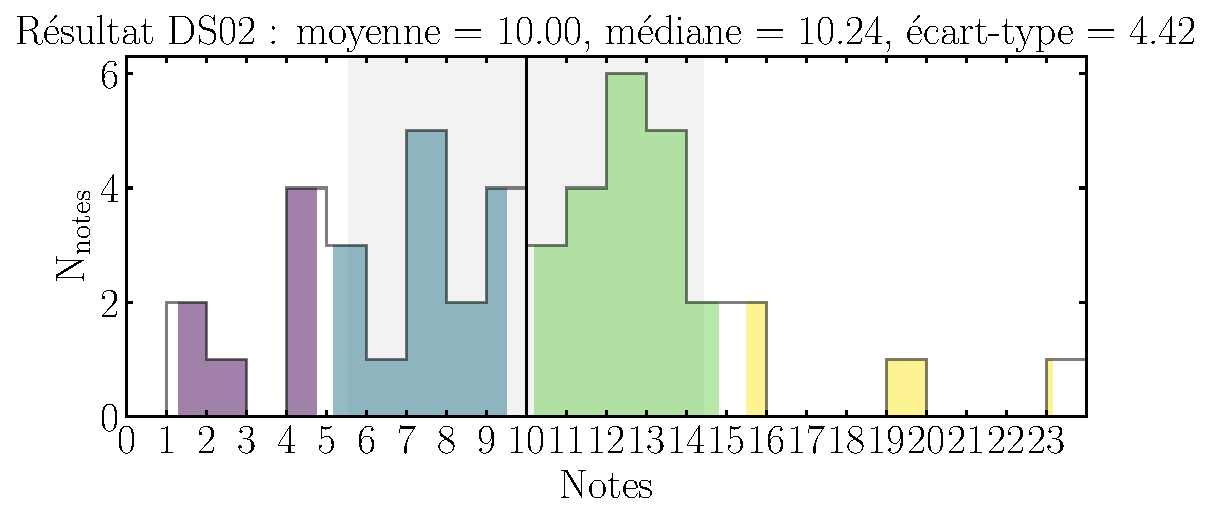
\includegraphics[width=.72\linewidth]{res_DS02.pdf}
\end{center}

\vfill

\end{document}
